\documentclass[article]{rian_article}

%%
% Atenção: Compilar com pdflatex !!!
%%

% Para colocar ao lado use \And para quebrar a linha use \AND
\author{Rian G.S. Pinheiro\\ \email{rian@ic.ufal.br}\And 
        Eric Coelho\\ \email{esc2@ic.ufal.br}}% \And
%         Terceiro Autor\\ \email{terceiro@ic.ufal.br} \AND
%         Quarto Autor\\ \email{quarto@ic.ufal.br} \And
%         Quinto Autor\\ \email{quinto@ic.ufal.br}}

% Autores separados por \&, se mais que 3 usar et al.
\Plainauthor{Rian Pinheiro \& Eric Coelho} %% comma-separated


\title{Algoritmo Genético BRKGA para o Problema de Empacotamento 2D 	Clássico com desempate}
\Plaintitle{Algoritmo Genético BRKGA para o Problema de Empacotamento 2D Clássico com desempate} %% Titulo sem formatação
\Shorttitle{BRKGA com desempate} %% a short title (aparece no topo das páginas)


%% an abstract and keywords
\Abstract{
	O \textit{Problema de empacotamento} (BPP) consiste em armazenar ortogonalmente um conjunto de itens na menor quantidade de caixas possível. A versão clássica assume que os itens têm orientação fixa e não pode haver sobreposição no empacotamento. O caso bidimensional generaliza o problema de empacotamento unidimensional clássico amplamente difundido na literatura, portanto, é da classe \NPhard~.
	Este trabalho apresenta um algoritmo genético de chaves aleatórias viciadas (BRKGA) para o \textit{problema de empacotamento bidimensional} (2BP), considerando os itens alocados com orientação fixa, baseando-se em chaves aleatórias como critério de desempate entre os espaços vazios ao inserir um novo item. O problema tem várias aplicações industriais, como corte, repartição e agendamento, relacionando-se a outros problemas complexos.
}

\Keywords{BRKGA, Bin Packing, 2BP, Meta-heurísticas}
\Plainkeywords{BRKGA, Bin Packing, 2BP, Meta-heurísticas} %% sem formatação


%% Informações do Trabalho
\Versao{1}
% \Versao{Final}
\Year{2020}
\Semestre{2}
\Month{Fevereiro}
\Submitdate{\today}
\Disciplina{Pesquisa Operacional}


%%%%%%%%%%%%%%%%%%%%%%%%%% PACOTES %%%%%%%%%%%%%%%%%%%%%%%%%%
\usepackage{amsmath}
\usepackage{bbm}
\usepackage{float}
\usepackage{subfig}
\usepackage{indentfirst}
\usepackage[T1]{fontenc}
\usepackage{url,bm}
\usepackage{textcomp}
\usepackage{graphicx}
\usepackage{amssymb}
\usepackage{anysize}
\usepackage{algpseudocode}
\usepackage{algorithm}
\usepackage{amsthm}
\usepackage{tikz}
\usepackage{enumerate}

%%%%%%%%%%%%%%%%%%%%%%%%% Comandos %%%%%%%%%%%%%%%%%%%%%%%%%%%%
\newcommand{\Cpp}{C\nolinebreak\hspace{-.05em}\raisebox{.4ex}{\tiny\bf +}\nolinebreak\hspace{-.10em}\raisebox{.4ex}{\tiny\bf +}~} 
\newcommand{\NPcom}{$\mathcal{NP}$-completo}
\newcommand{\NPhard}{$\mathcal{NP}$-Difícil}
\newtheorem{teorema}{Teorema}[section]
\floatname{algorithm}{Algoritmo}
\newenvironment{prova}{\begin{proof}[\bf\textsc{Prova.}]}{\end{proof}}



\begin{document}

% Este exemplo foi publicado no SBPO 2015.
\section{Introdução}

O \textit{problema de empacotamento clássico bidimensional} (2BP) consiste em empacotar ortogonalmente um conjunto de $n$ itens em forma de retângulos caracterizados por sua altura $h_{i}$ e largura $w_{i}$, $i \in \{1, 2, 3, ... , n\}$, no menor número possível de caixas homogêneas de altura $H \geq h_{i}$ e largura $W \geq w_{i}$. A quantidade de caixas é ilimitada e os itens não podem ser alocados com sobreposição.

\begin{figure}[hbt]
\centering
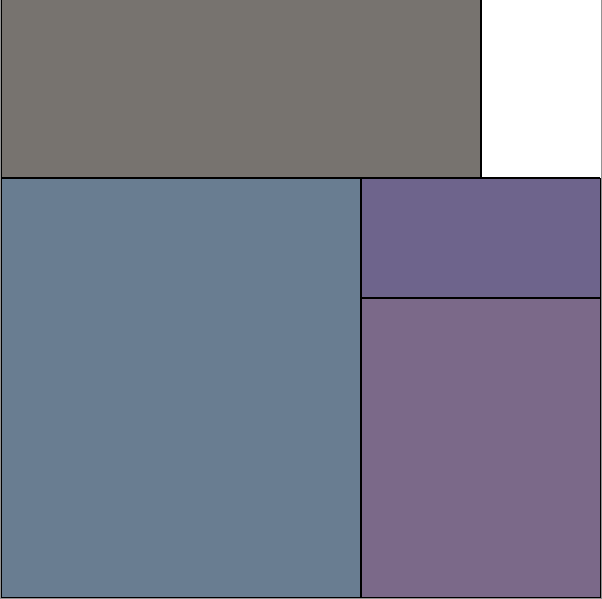
\includegraphics[width=0.3\textwidth]{figs/ex_instance_1.png}\hspace{0.1\textwidth}
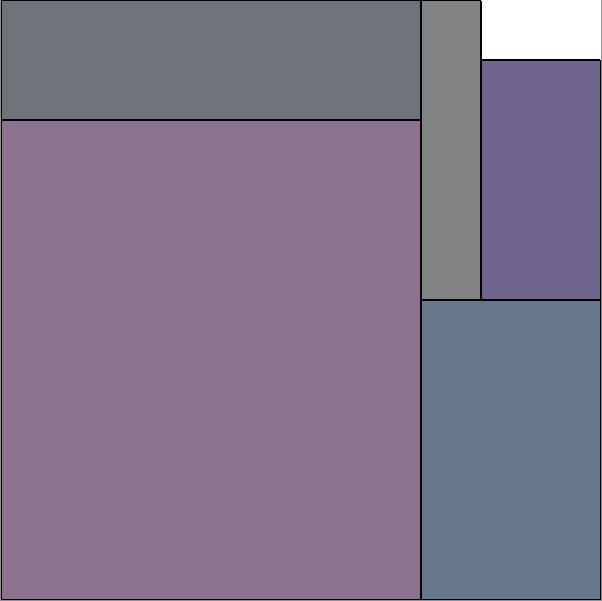
\includegraphics[width=0.33\textwidth]{figs/ex_instance_2.png}
\caption{Exemplo do 2BP.} \label{fig:ex}
\end{figure}
 
Exemplo de instância do 2BP na Figura~\ref{fig:ex}

\subsection{Aplicações}
Várias aplicações industriais têm interesse particular no 2BP. Dentre elas, podemos citar aplicações de carregamento de objetos sensíveis em caminhões e aviões, armazenamento de mercadorias, empacotamento de encomendas, reconfiguração dinâmica de hardware e carregamento de paletes. Por exemplo, quando um editor precisa preencher as páginas de um jornal, ele tem que considerar como rearranjar e posicionar os retângulos de textos e propagandas, ou seja, empacotamento de itens em que uma de suas faces deve permanecer obrigatoriamente para cima. Apesar de ser uma simplificação do mundo real, as heurísticas que encontram boas soluções para os problemas de empacotamento na versão clássica são aplicadas com sucesso em versões com restrições adicionais que modelam situações reais [Parreño et al., 2010b; Kang et al., 2012; Li et al., 2014; Saraiva et al., 2015; Boyar et al., 2016; Moura e Bortfeldt, 2017]. Além disso, o problema aparece como subparte de outros problemas mais complexos como os de agendamento, corte e particionamento.
\section{Algoritmo BRKGA}\label{sec:corte}
O algoritmo genético de chaves aleatórias viciadas (BRKGA) foi introduzido por \citet{resende2011} para problemas de otimização combinatória. Esta meta-heurística é uma variante do algoritmo genético de chaves aleatórias (RKGA) [Bean, 1994]. 
A ideia principal é evoluir uma população codificada em cromossomos. Cada indivíduo é representado por uma sequência de chaves aleatórias ou random-keys, na forma de vetores de números reais no intervalo [0, 1].
O componente chamado decodificador deve ser implementado para cada problema. Este componente deve receber um vetor de random-keys para fornecer uma representação do indivíduo que pode ser avaliada. Para o 2BP, o decodificador é composto de dois componentes: um método de ordenação e um algoritmo guloso para realizar o empacotamento dos itens:

O método de ordenação deve receber um vetor com n random-keys, um para cada item da instância, para fornecer uma permutação de itens. As chaves devem ser ordenadas de modo que o item $a_{i}$ é empacotado antes do item $a_{j}$ se e somente se $k_{i} < k_{j}, {i}, {j} \in \{1, ..., {n}\}$, onde $k_{i}$ e $k_{j}$ são as respectivas random-keys associadas.
O algoritmo guloso constrói uma solução iterativamente, recebendo uma permutação de inteiros que representa a sequência em que os itens serão empacotados sequencialmente.

Após o processo de ordenação, a permutação associada ao cromossomo do indivíduo é passada como parâmetro de entrada para o algoritmo guloso, denominado Distance to the Front-Top-Right Corner (DFTRC) \citep{resende2013}. Sabendo que uma caixa aberta da solução corrente é uma que contém itens empacotados, para cada iteração {k} do DFTRC, o algoritmo busca por espaços que possam conter o item  $a_{k}, {k} \in \{1, ..., {n}\}$ a ser empacotado. Se nenhuma caixa aberta até o momento pode conter o item, então uma nova caixa é introduzida na solução com $a_{k}$ empacotado. No passo de empacotamento, áreas maximais são utilizadas para modelar o espaço vazio de cada caixa aberta. 

Uma área maximal é a maior área retangular possível dentro da caixa aberta que não há itens. Todas as áreas maximais que podem conter o item da iteração corrente são candidatas para a escolha da localização do empacotamento. O DFTRC seleciona a área maximal que maximiza a distância entre o canto superior direito frontal do item para o respectivo canto superior direito frontal da caixa.

Caso haja empate entre as áreas maximais, um segundo vetor de random keys é utilizado para selecionar entre as duas melhores áreas maximais.


O Algoritmo~\ref{alg:const} apresenta a visão geral do procedimento de empacotamento.

\begin{algorithm}[hbtp]
\caption{Placement}
\label{alg:const}
\begin{algorithmic}[1]
\footnotesize
\Procedure{Placement}{$BPS,TB$}
	\State{Inicialize $B$ com as caixas abertas}\Comment{comentario}
	\State{Inicialize $NB$ com o número de caixas abertas}
	\For{$i \in \{1, ..., {n}\}$}
		\State{$BoxToPack \gets BPS\{i\}$}
		\State {$SelectedBin \gets 0$}
		\For{$k \in \{1, ..., {NB}\}$}
			\State{$BestEMSList \gets$ \textsc{DFTRC}($k, BoxToPack$)}
			\If{$BestEMSList > 0 $}
				\State {$SelectedBin \gets k$}
				\State \textbf{break}
			\EndIf
		\EndFor
		\If{$BestEMSList \neq \emptyset$}
			\State{$EMSselected \gets$ \textsc{EMSSelector}($TB_i, BestEMSList$)}
		\Else
			\State{$NewBin \gets NB + 1 $}
			\State{$B \gets B \cup {NewBin} $}
			\State{$NB \gets NB + 1 $}
			\State{$EMSSelected \gets NewBin_0 $}
		\EndIf
		\State{Calcula a posição do item na caixa a partir de $EMSSelected$}
		\State{\textsc{DifferenceProcess}($SelectedBin, BoxToPack$)}
	\EndFor
\EndProcedure
\end{algorithmic}
\end{algorithm}

\section{Experimentos Computacionais}
A base de testes utilizada neste trabalho é composta por 500 instâncias do 2BP detalhadas em \citet{martello1998}. As instâncias são organizadas em 10 classes com 10 instâncias para cada quantidade de itens ${n} \in \{20, 40, 60, 80, 100\}$. Esta base se trata de uma extensão das instâncias propostas em \citet{wang1987}.

\subsection{Ferramentas}\label{sec::ferramentas}

O BRKGA proposto foi implementado utilizando a linguagem de programação C++11, e foi compilado com o GCC do GNU Compiler Collection. O ambiente computacional utilizado em todos os testes neste trabalho consiste de um desktop munido da seguinte configuração: processador AMD FX-6300 @3.5 GHz, 8 GB de memória RAM e sistema operacional Ubuntu 18.04. A Tabela~\ref{tab:params} relaciona os parâmetros calibráveis do BRKGA com os respectivos valores.

\begin{table}[htb]
	\caption{Parâmetros do BRKGA}
	\label{tab:params}
	\centering
	\footnotesize
	\begin{tabular}{|l|c|c|c|c|}
		\hline
		Instância	&Exato    &\citep{chan1997}    & GRASP	& GRASP+SP	\\ \hline
		i1	        &17       &17	  & 17		&17		\\ \hline
		i2	        &20       &20	  & 20		&20		\\ \hline
		i3	        &36       &36	  & 36		&36		\\ \hline
		i4	        &34       &34	  & 34		&34		\\ \hline
	\end{tabular}
\end{table}


\subsection{Resultado}

TABELA de RESULTADOS DA EXECUÇÃO

A tabela apresenta a instância, seguida do número de edições encontradas pelo algoritmo exato \citet{martello2002}, a solução encontrada na literatura \citep{chan1997}, juntamente com a solução do GRASP proposto e do GRASP+SP.
Observa-se que o algoritmo GRASP encontra o valor ótimo em todas as instâncias com exceção da \texttt{i11}.
Já o GRASP+SP, encontrou a solução ótima em todas as instâncias.


A Tabela~\ref{tab:tempo} apresenta a instância, junto com o tempo de execução do algoritmo de \citet{martello2002}, o tempo de execução do GRASP proposto e o tempo de execução do GRASP+SP.
Note que, o tempo de GRASP proposto foi muito inferior ao tempo de execução da literatura.
Observa-se ainda que os tempos do GRASP e do GRASP+SP foram próximos.
Além disso, algoritmo de foi executado em uma máquina Intel Core i7-2600 com 3.40GHz, enquanto que o deste artigo foi executado em uma máquina Intel Core i7-4500U com 1.80GHz.


No que diz respeito ao pré-processamento da Seção~\ref{sec:corte}, ele se mostrou eficaz em instâncias esparsas, porém sem muita efetividade para as instâncias densas.

 \begin{table}[hbtp]
\caption{Tempos do GRASP e GRASP+SP}
\label{tab:tempo}
\centering
\footnotesize
\begin{tabular}{|l|c|c|c|}
\hline
Instância	  & \citep{zudio2018}	&GRASP    & GRASP+SP	   \\ \hline
i1	  & 7,23	&0,26	  & 0,30	  \\ \hline 
i2	  & 7,00	&0,21	  & 0,24	  \\ \hline 
i3	  & 10,09	&0,39	  & 0,45	  \\ \hline 
i4	  & 9,97	&0,35  	  & 0,41	  \\ \hline 
i5	  & 12,90	&0,41     & 0,46	  \\ \hline 
i6	  & 13,89	&0,48     & 0,49	  \\ \hline 
i7	  & 7,88	&0,49     & 0,52	  \\ \hline 
i8	  & 13,13	&0,39     & 0,42	  \\ \hline 
i9	  & 12,53	&0,47     & 0,50	  \\ \hline 
i10	  & 20,31	&0,98     & 1,09	  \\ \hline 
i11	  & 23,41	&1,35     & 1,17	  \\ \hline 
i12	  & 24,50	&1,40     & 1,26	  \\ \hline 
i13	  & 47,19	&2,66	  & 2,39	  \\ \hline 
i14	  & 48,24	&2,82	  & 2,78	  \\ \hline 
i15	  & 65,95	&3,27	  & 3,25	  \\ \hline
i16  	& 3,40		& 0,09	   & 0,10	  \\ \hline
i17  	& 4,02		& 0,05	   &  0,05	  \\ \hline
i18  	& 5,26		& 0,12	   &  0,14	  \\ \hline
i19  	& 5,28		& 0,06	   &  0,08	  \\ \hline
i20  	& 7,05		& 0,36	   &  0,39	  \\ \hline
i21  	& 31,80		& 0,15	   &  0,14	  \\ \hline
i22  	& 24,27		& 0,17	   &  0,14	  \\ \hline
i23  	& 26,45		& 1,71	   &  1,48	  \\ \hline
i24  	& 25,56		& 3,28	   &  3,24	  \\ \hline
i25  	& 26,48		& 0,16	   &  0,19	  \\ \hline
i26  	& 43,42		& 2,95	   &  3,05	  \\ \hline
i27  	& 51,80		& 0,20	   &  0,22        \\ \hline
i28  	& 77,30		& 15,52	   &  16,09	  \\ \hline
i29  	& 71,91		& 13,73	   &  13,65	  \\ \hline
i30  	& 77,21		& 0,34	   &  0,37	  \\ \hline
\end{tabular}
\end{table}


\section{Conclusão}
Este trabalho aplicou a heurística BRKGA para o problema clássico de empacotamento bidimensional, sem considerar a rotação dos itens. O algoritmo é baseado na meta-heurística BRKGA, e utiliza um algoritmo guloso para empacotar os itens. Através de um conjunto de 500 instâncias, as quais compõem a base de teste padrão para vários trabalhos encontrados na literatura, o BRKGA foi comparado com outras abordagens encontradas na literatura. Os experimentos mostraram que o BRKGA proposto aliado com o critério de desempate obtém resultados equivalentes ou melhores aos reportados na literatura.

PROPROSTAS
Para trabalhos futuros serão propostas novas melhorias que acelerem o método, como por exemplo novo módulos exatos.
Pretende-se estender o pré-processamento proposto para os coasos em que a biclique não é completa.
Além disso, um estudo mais aprofundado com relação à elaboração de instâncias mais difíceis.
Com relação a meta-heurística, pode-se pensar em novos métodos construtivos e novas buscas locais.


\bibliography{refs2}
\end{document}
